\section{Results}
\subsection{$H_{1a}$ and $H_{1b}$}

To test $H_{1a}$, we first establish a model with 50 agents, 5 issues, and an
openness parameter of 0.40. In order to measure the impact of varying edge
probability on average assortativity across all issues, we run each combination
of parameters 20 times starting with an edge probability of 0.05 and ending
with an edge probability of 0.95, in increments of .05. The results of this
model run are shown in Figure~\ref{H1a_plot}.

\begin{figure}
\centering
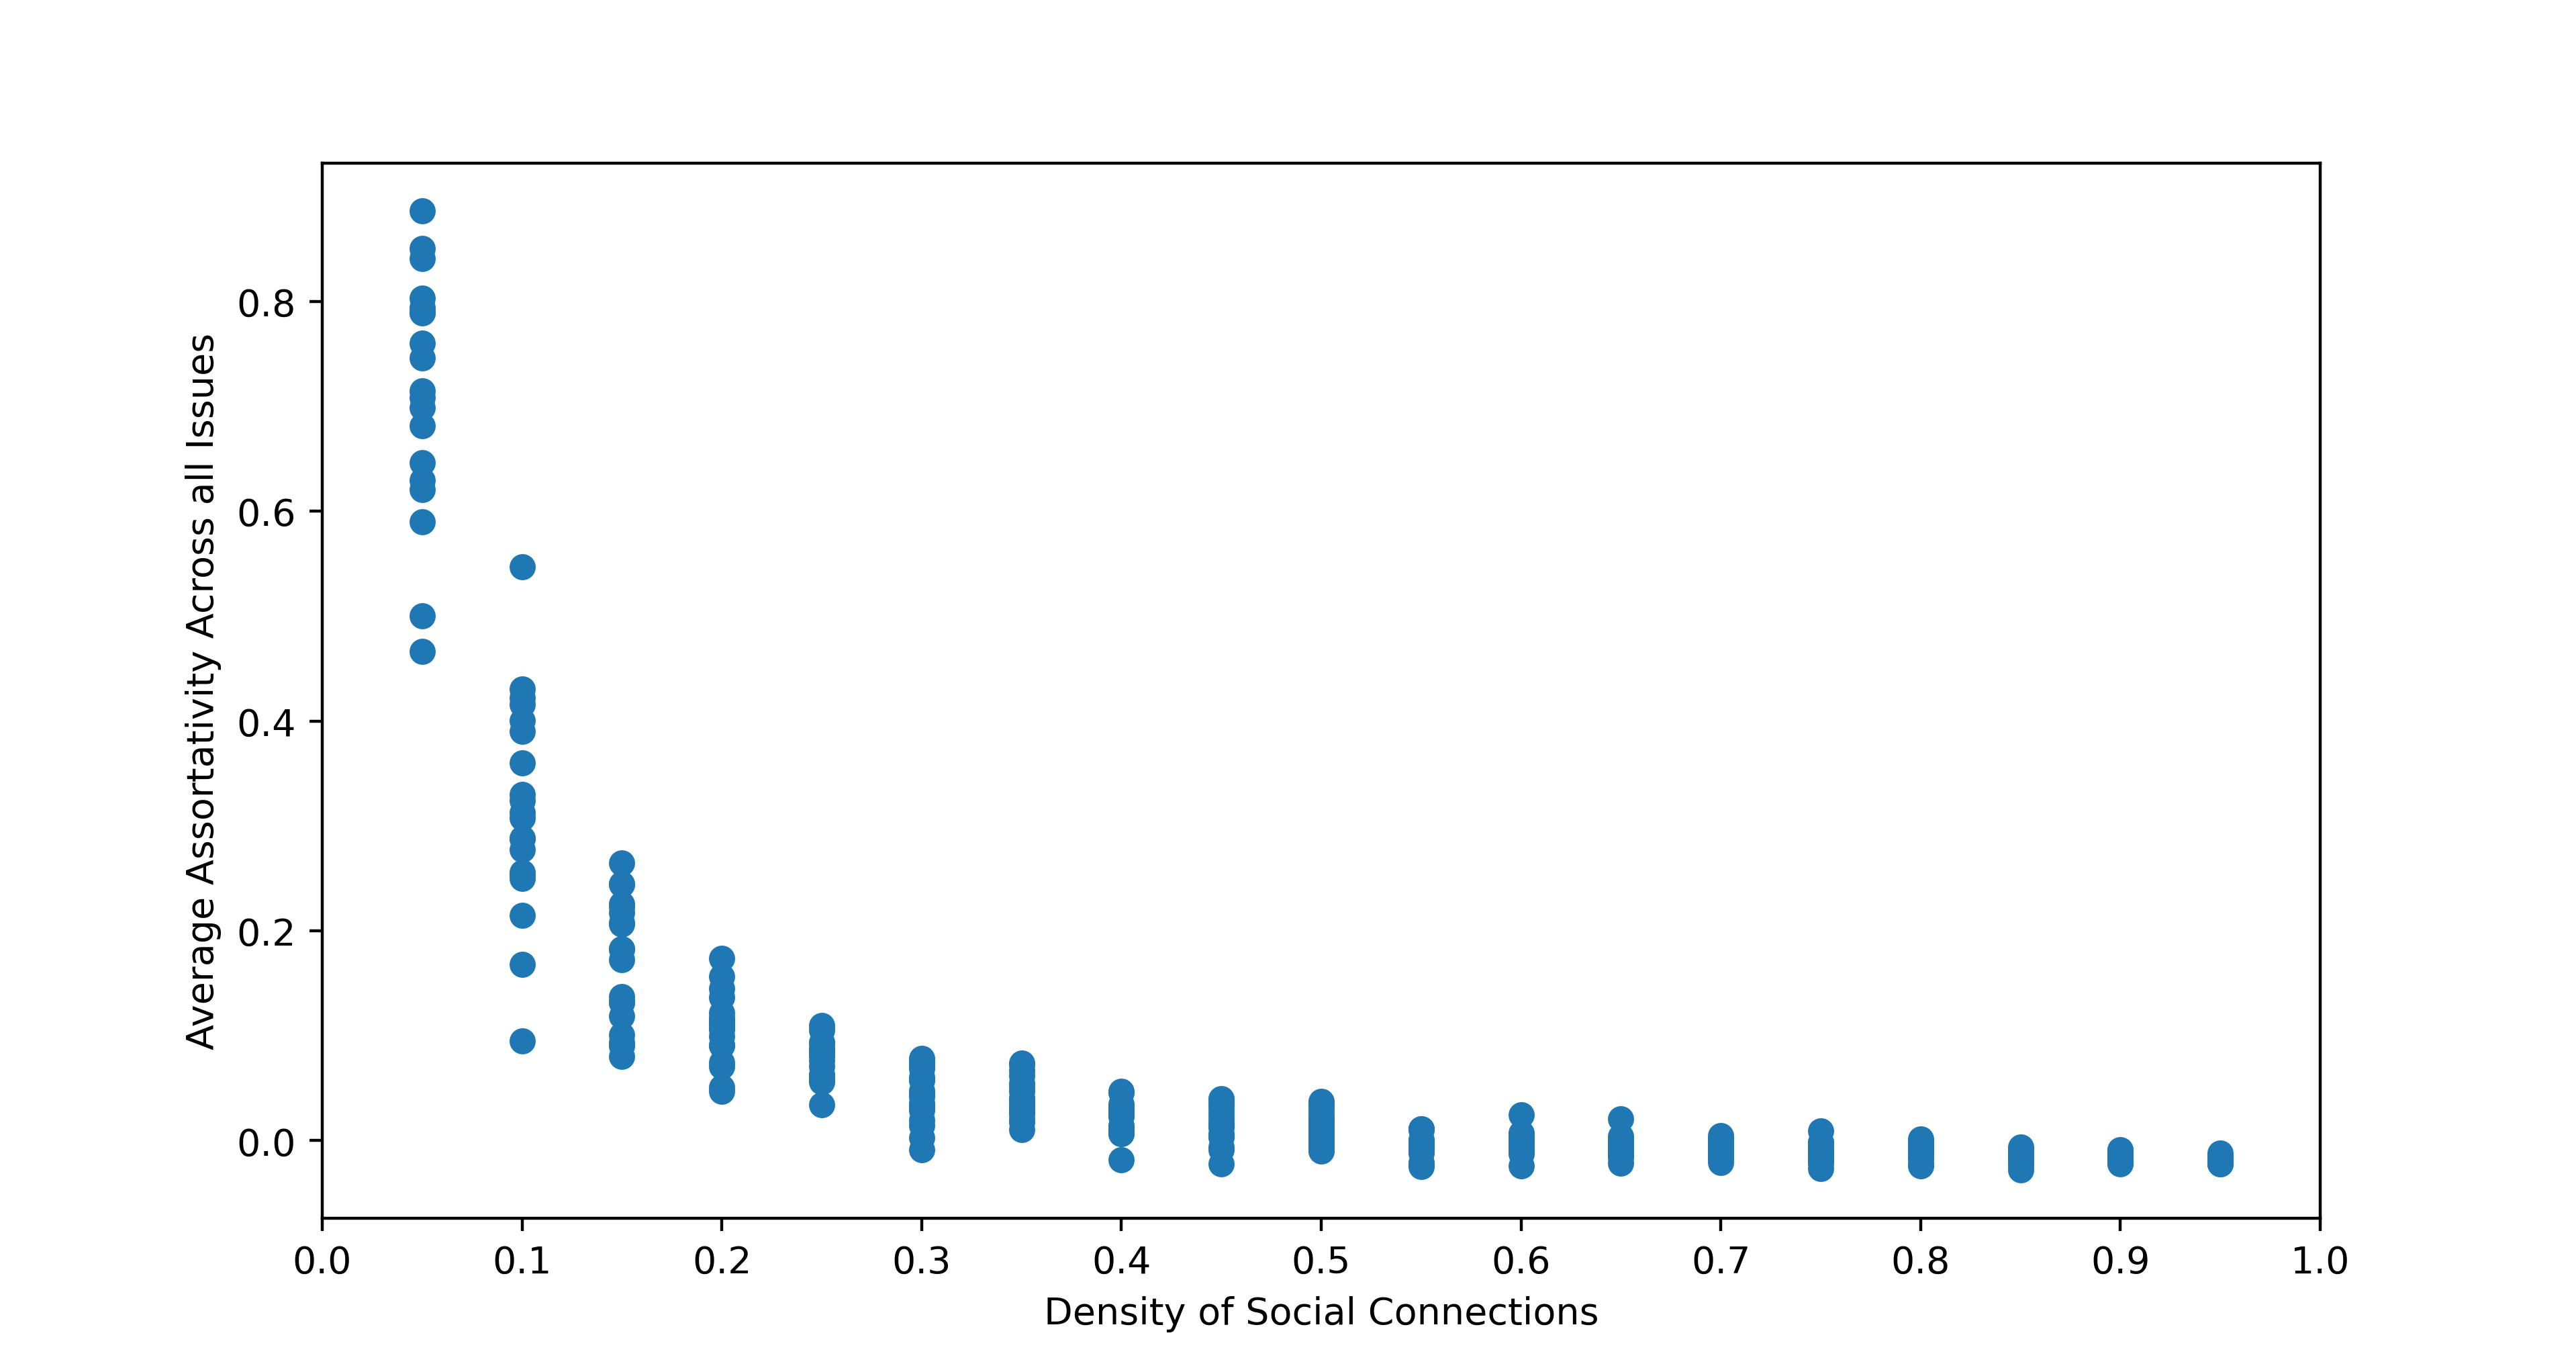
\includegraphics[width=1.0\columnwidth]{./Graphs/Assort_edge.png}
\caption{Average Assortativity across all Issues and Edge Probability}
\label{H1a_plot}
\end{figure}

We see that as the edge probability (or density of social connections)
increases, the average assortativity across all issues decreases. This is the
exact opposite of our hypothesis. One possible explanation for this result is
that when connections are more dense, there is a higher chance that agents will
be exposed to a more diverse set of opinions. There is thus a higher chance
that agents will be pulled to the `average` opinion for a given issue, which
would produce lower assortativity. From this finding, we may be able to infer
that societies where individuals are more densely connected may experience
less polarization than more sparsely-connected societies do.

In addition to the negative correlation between density of social connections
and polarization, we also see that the relationship between these two variables
appears negative-exponential in nature. The variance was too high, however, for
us to draw a solid conclusion on whether the relationship truly conforms to a
negative-exponential, a power-law, or any other standard distribution.

To test $H_{1b}$, we first establish a model with 50 agents, 5 issues, and an
edge probability of 0.50. In order to measure the impact of varying the
openness parameter on average assortativity across all issues, we ran each
combination of inputs 20 times with an openness parameter ranging from 0.05 to
0.95 in increments of .05. The results of this model run are shown in
Figure~\ref{H1b_plot}. As is depicted, there is no obvious relationship at all
between the openness parameter and the average assortativity across all issues. 

\begin{figure}
\centering
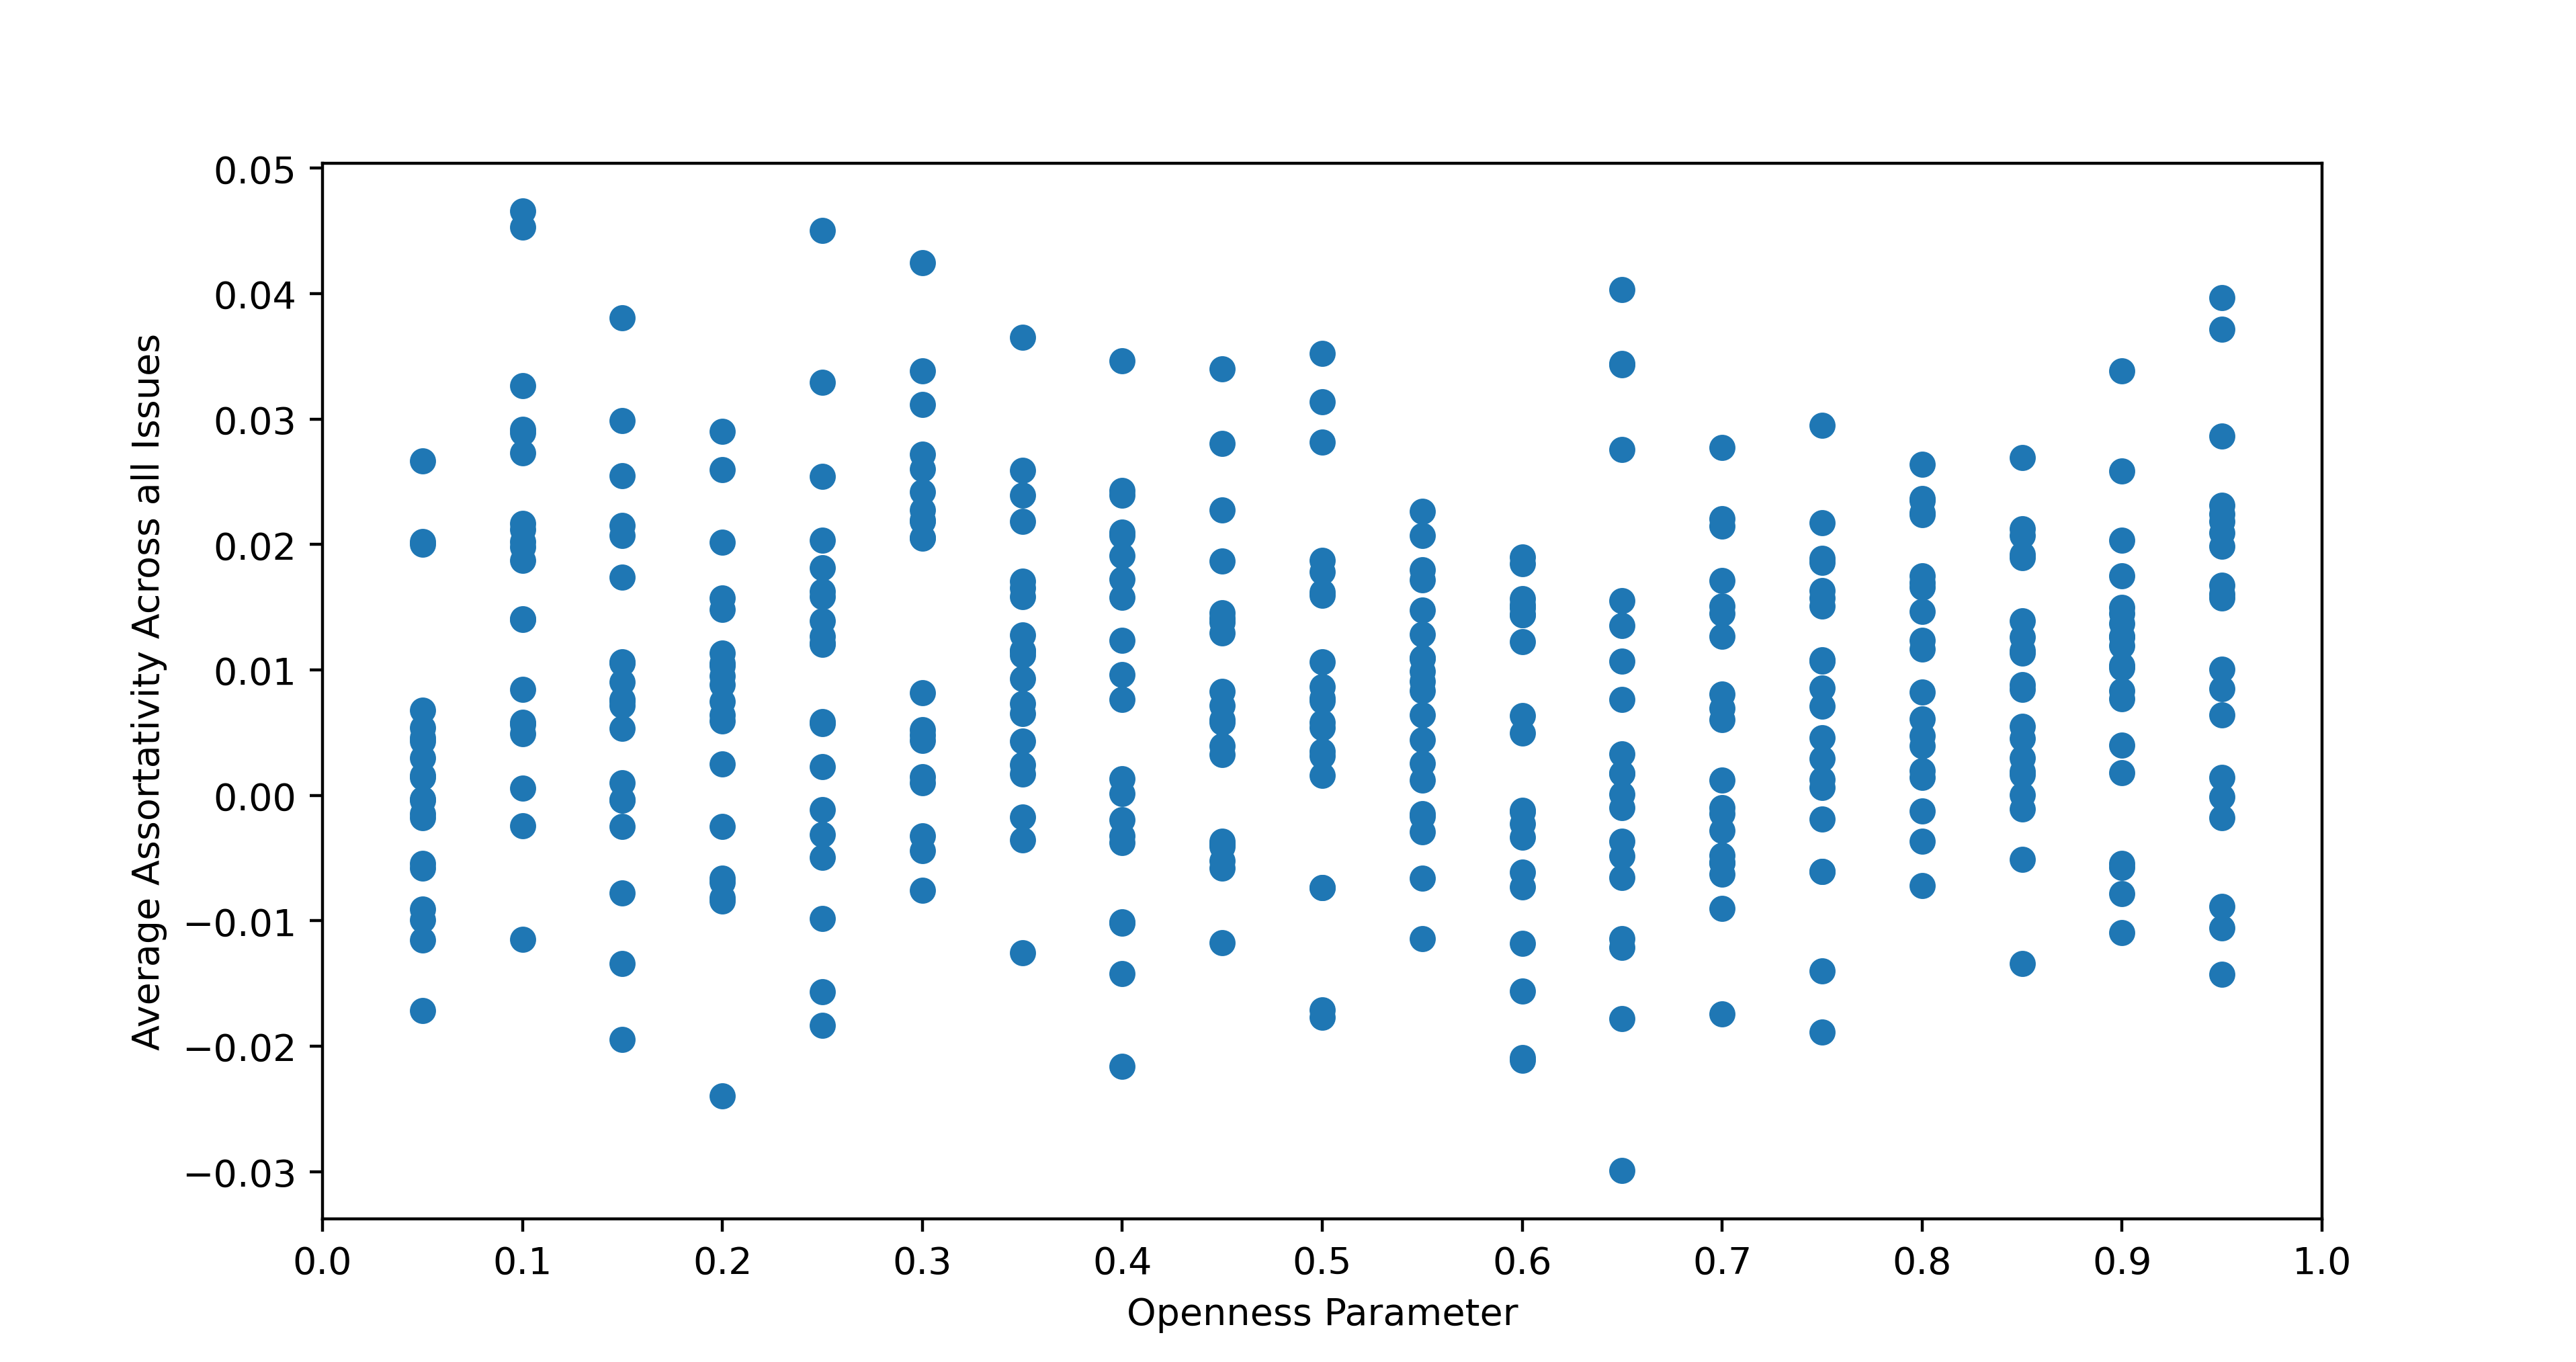
\includegraphics[width=1.0\columnwidth]{./Graphs/Assort_openness.png}
\caption{Average Assortativity across all Issues and Openness Parameter}
\label{H1b_plot}
\end{figure}

This is an interesting result. Agents in the model are influenced when they are
close in opinion (within our openness parameter) to another agent on the same
issue. Therefore, we believed that openness would play a role in determining the assortativity of a society. 
It should be noted that we tested this hypothesis with multiple different values of the edge probability (0.15,
0.40, and 0.50), to ensure that the edge probability was not having an impact
on our results. Even still, we hope to investigate this hypothesis further in future research. 

\subsection{$H_{2a}$ and $H_{2b}$}

To test $H_{2a}$, we establish a model with 50 agents, 5 issues, and an
openness parameter of 0.30. First, we ran a parameter sweep varying the edge
probability from 0.05 to 0.95 to measure the impact of this parameter on the
number of opinion clusters. The results of this parameter sweep are shown in
Figure~\ref{H2a_plot_big}.

\begin{figure}
\centering
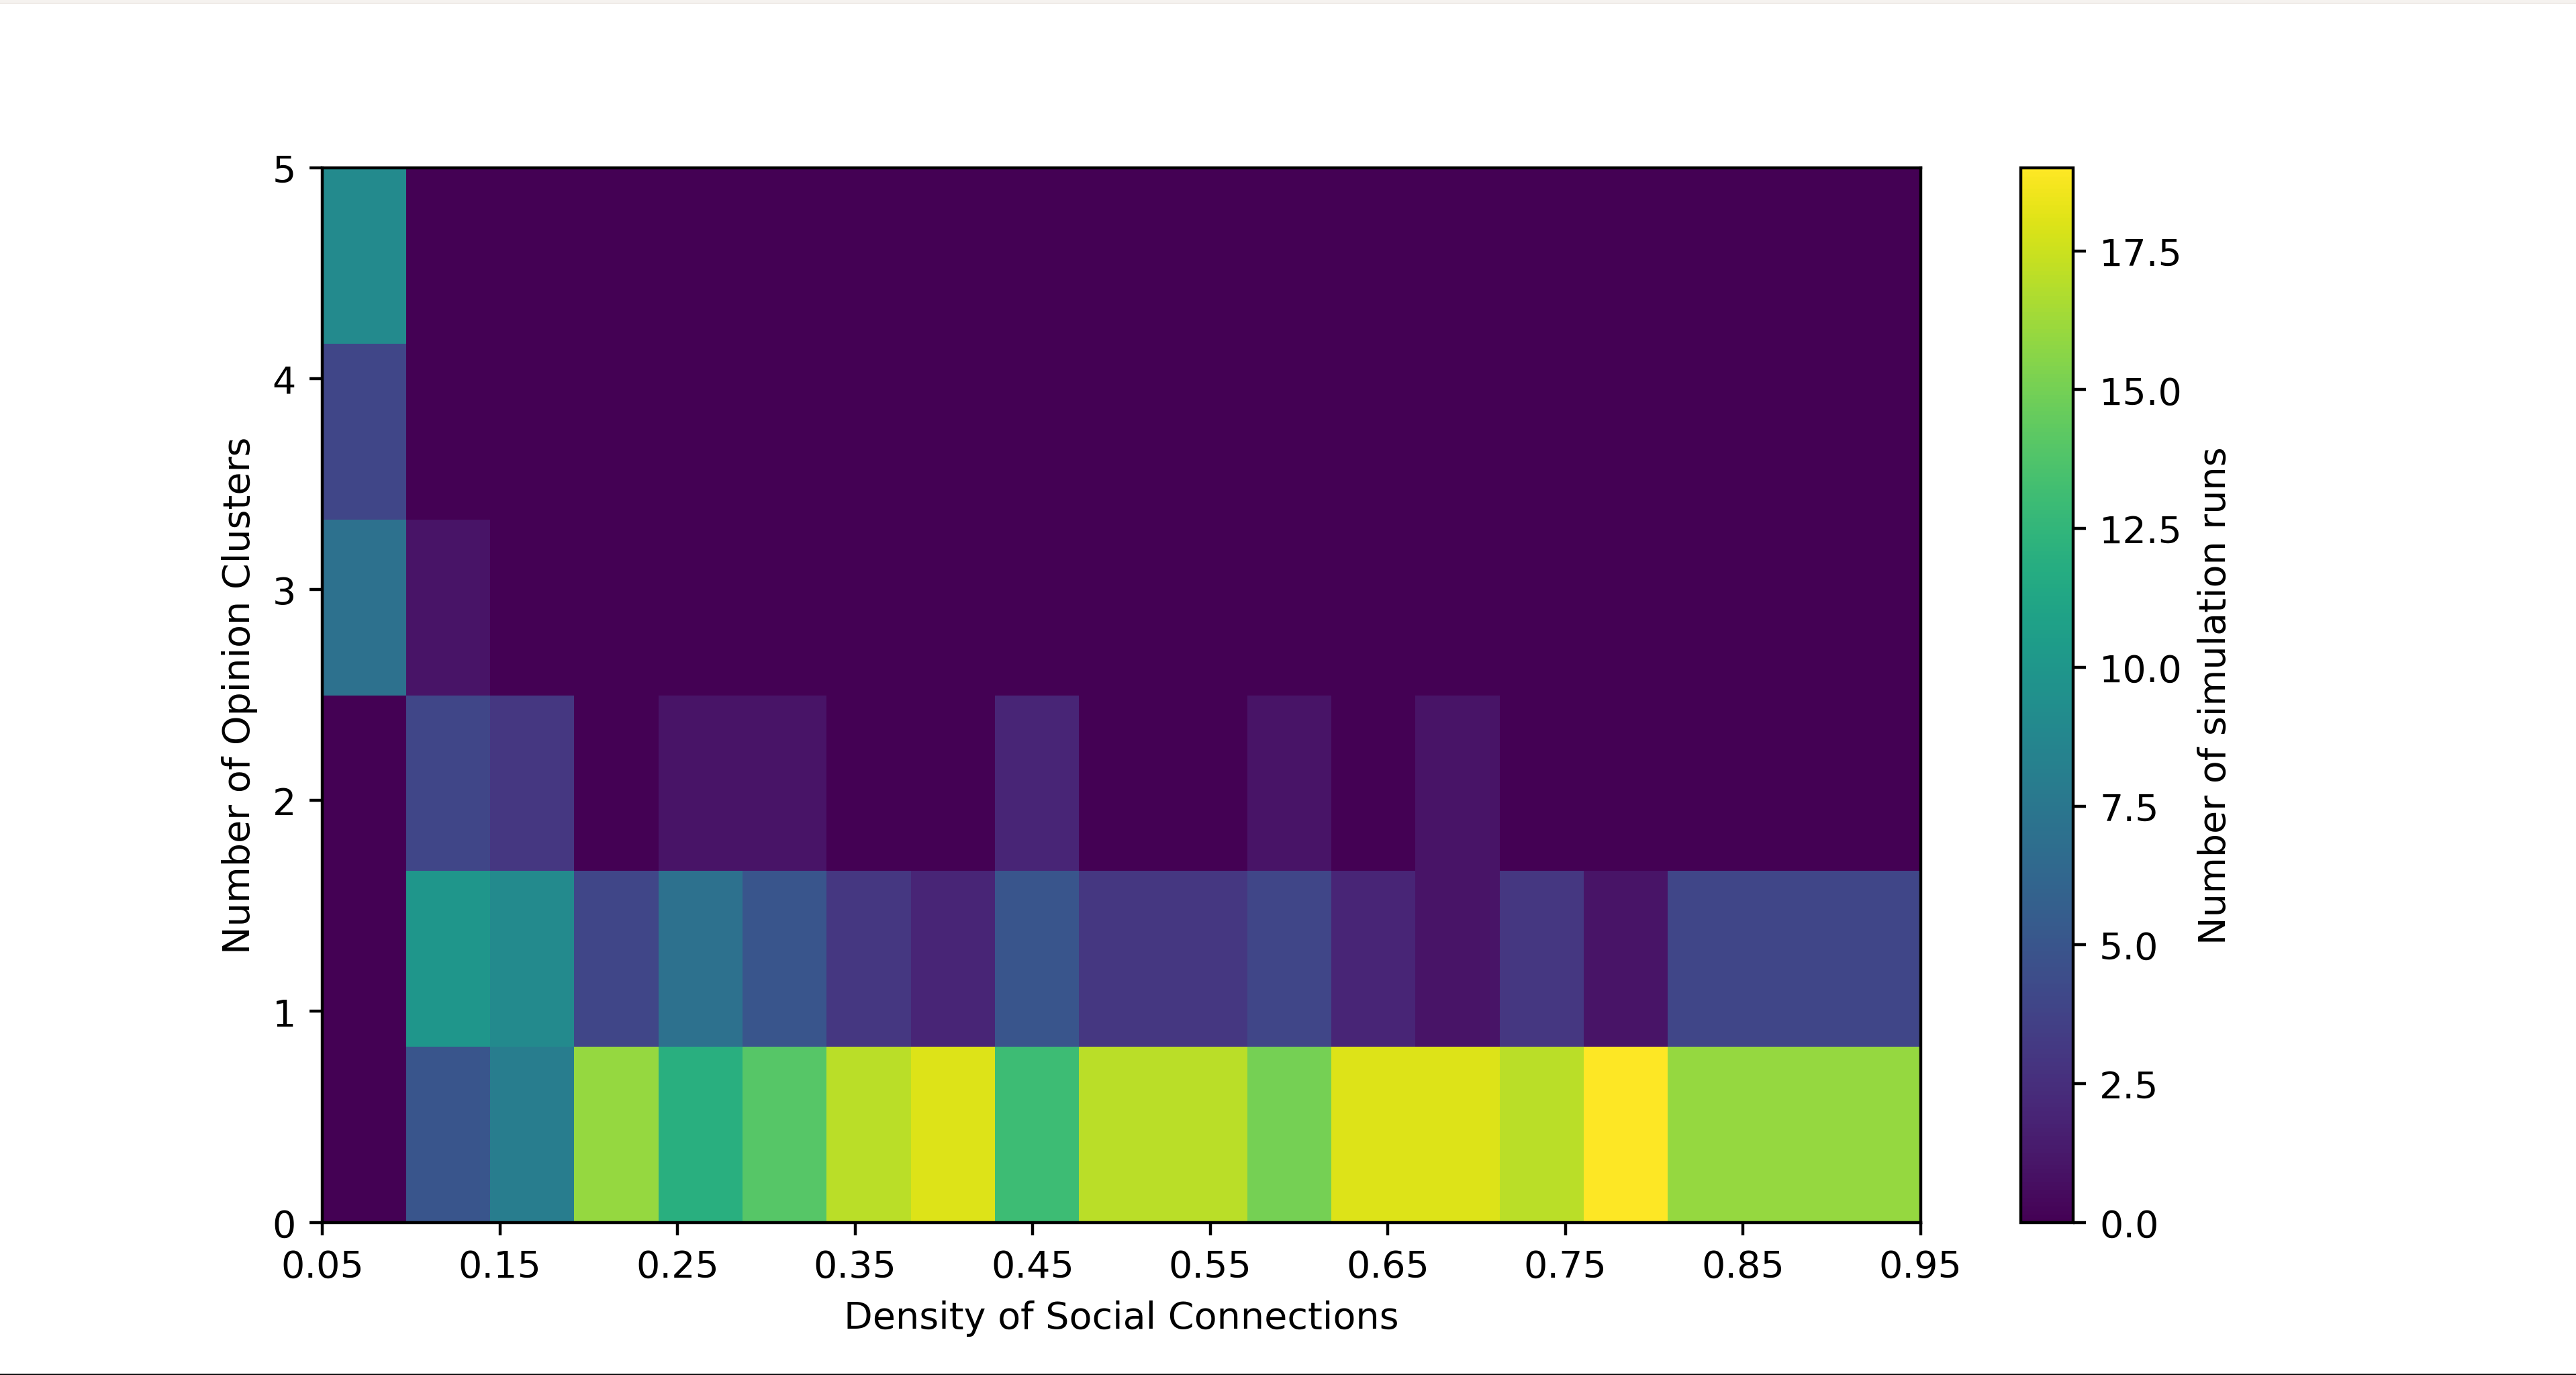
\includegraphics[width=1.0\columnwidth]{./Graphs/ClusterEdge/Cluster_edgeBig.png}
\caption{Number of Opinion Clusters and Edge Probability (0.05 - 0.95)}
\label{H2a_plot_big}
\end{figure}

We noticed that as with $H_{2a}$, there appears to be a tipping point with the
number of opinion clusters and the edge probability. To further explore this
hypothesis, we ran another parameter sweep, this time varying the edge
probability from 0.05 to 0.40 incrementing by 0.01 for each suite of 20 model
runs. The results of this parameter sweep are depicted in
Figure~\ref{H2a_plot_small}.

\begin{figure}
\centering
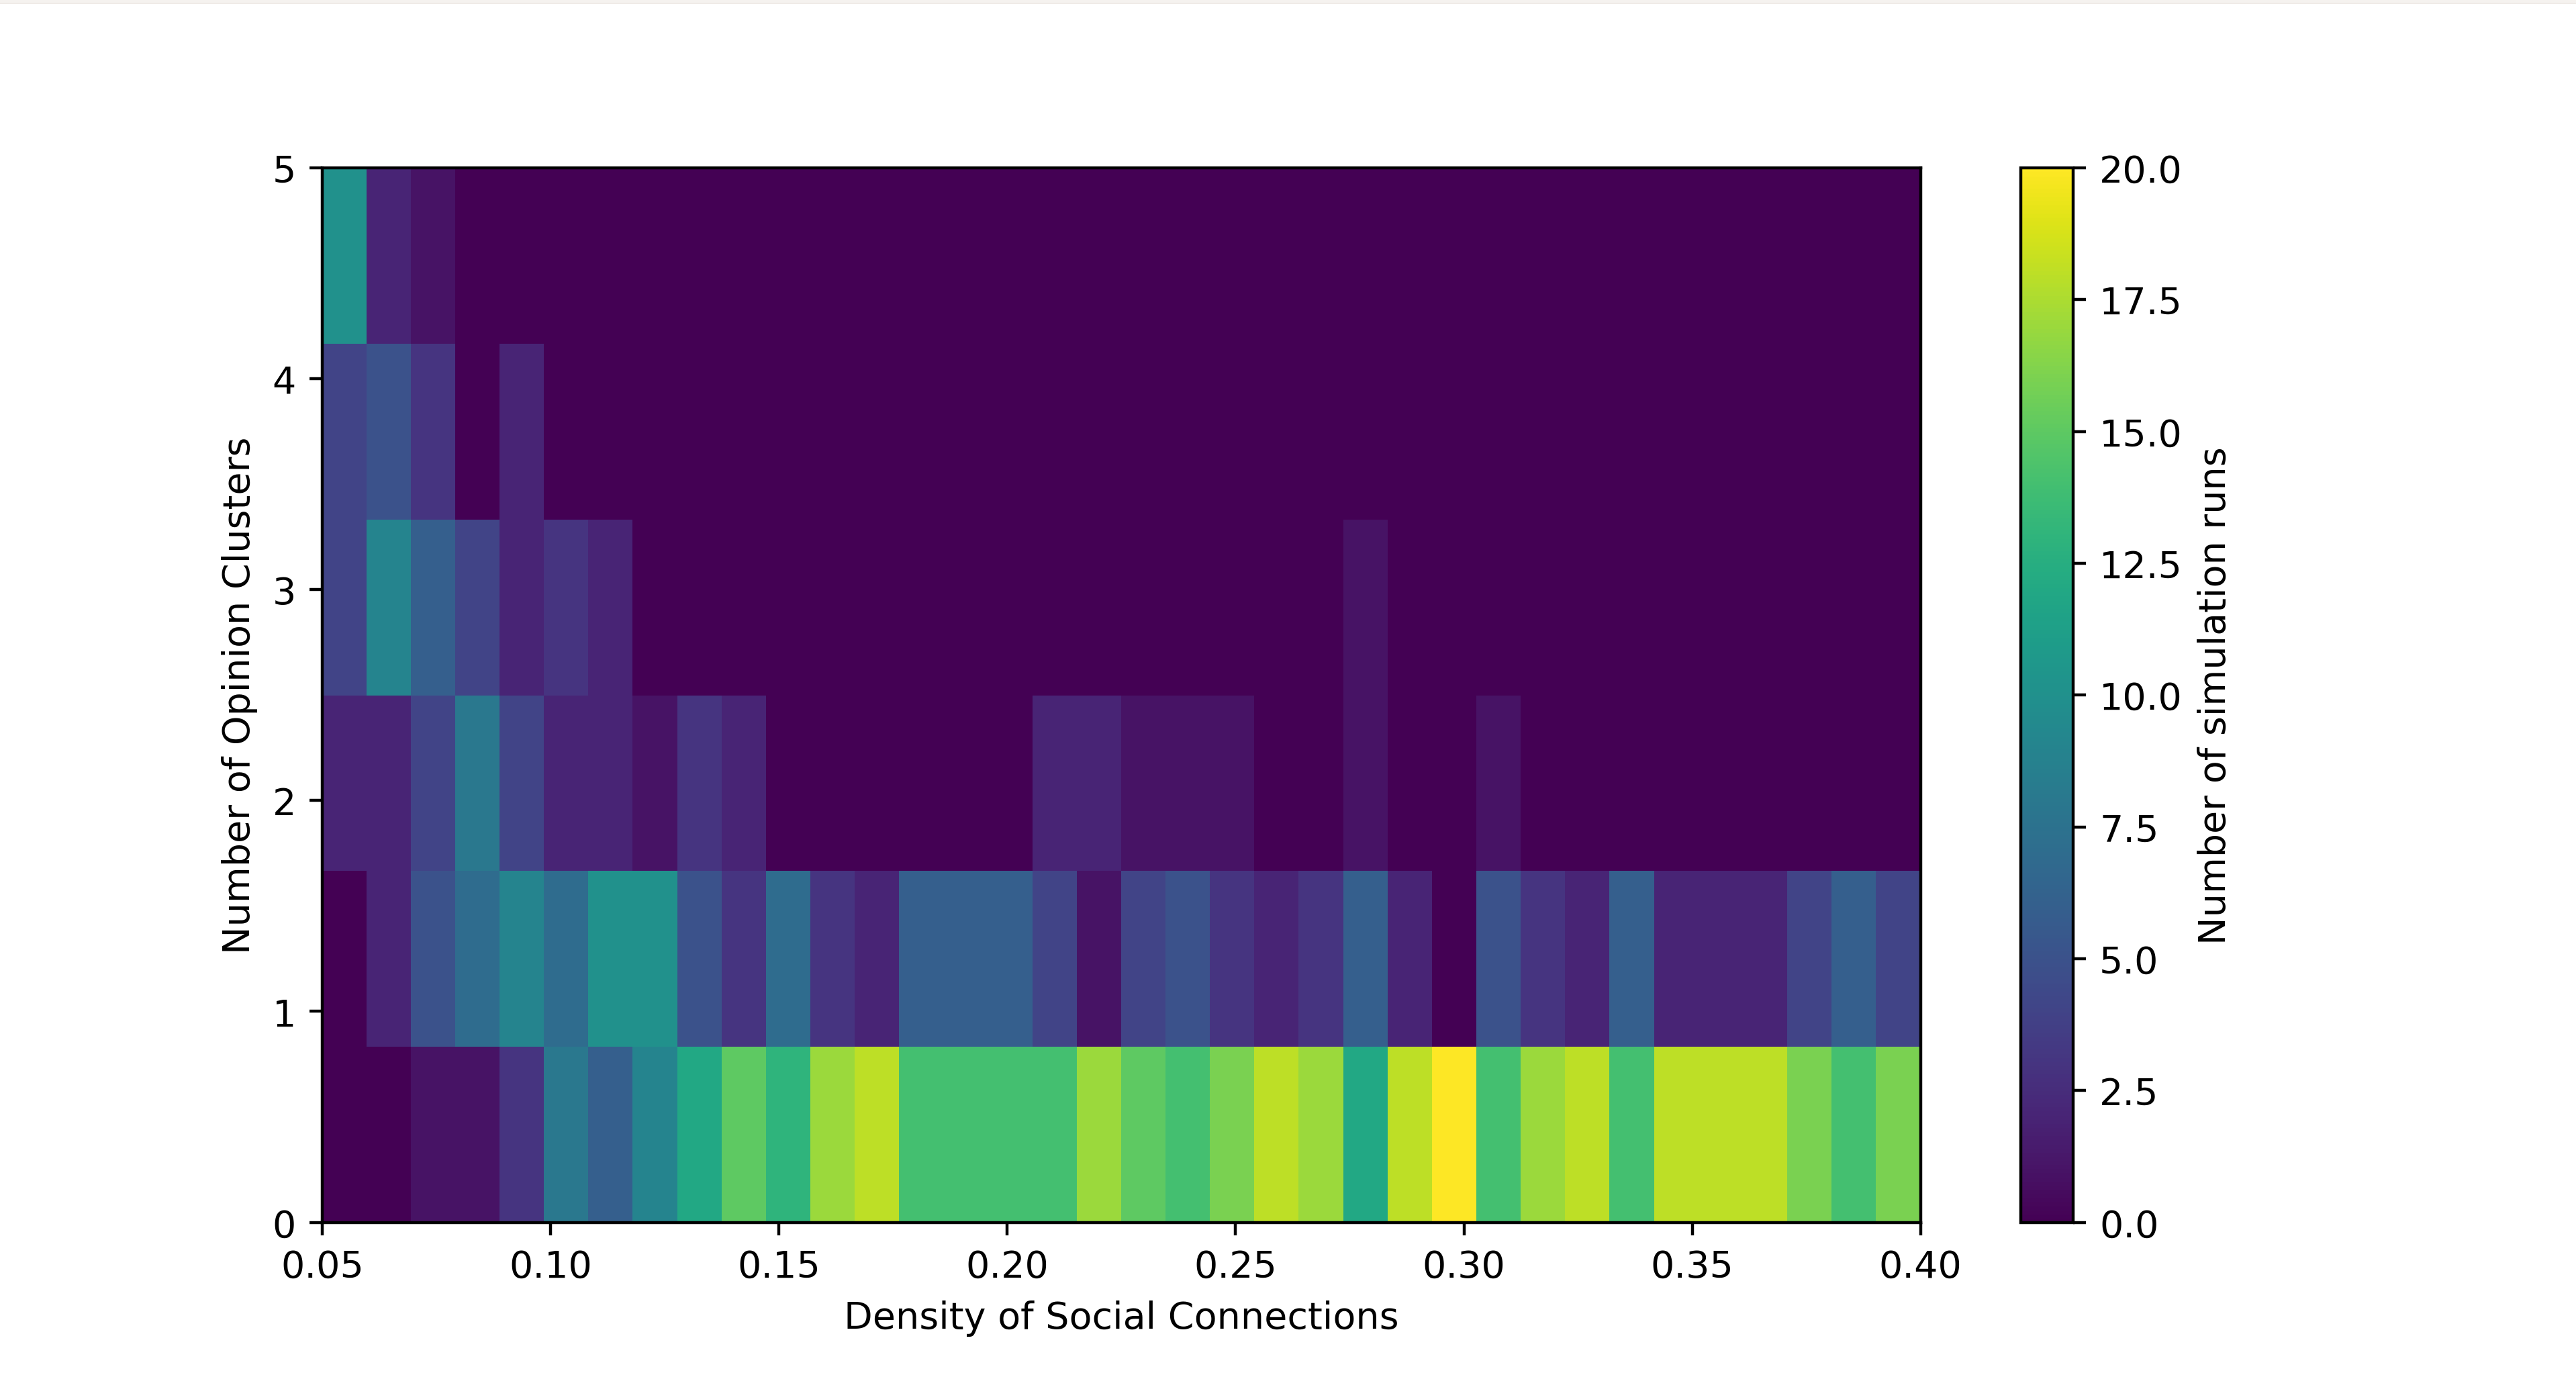
\includegraphics[width=1.0\columnwidth]{./Graphs/ClusterEdge/Cluster_edgesmall.png}
\caption{Number of Opinion Clusters and Edge Probability (0.05 - 0.40)}
\label{H2a_plot_small}
\end{figure}

Our results confirm $H_{2a}$; the number of opinion clusters and edge probability have a negative relationship. We believe this may be explained by the implications of a high density for a graph of nodes. For example, when a graph of 50 nodes has a density of 0.05, the average number of social connections will be 2.5. We are able to calculate the average number of social connections by multiplying the chance there will be an edge between any two nodes (edge probability) and the number of nodes. When the edge probability, or density of the graph, increases slightly to 0.2, the average number of social connections will rise to 10 connections. As a result, the geodesic distance between two nodes decreases rapidly because each node is proportionately connected to more nodes in the graph. This may reveal why we saw that only a certain level of density is required for the number of opinion clusters to drop sharply. Undeniably, a tipping point exists with the number of opinon clusters when increasing the density of an Erd\"{o}s-R\'{e}nyi graph in our model.  

To test $H_{2b}$, we establish a model with 50 agents, 5 issues, and an edge
probability of 0.50. First, we ran a parameter sweep varying the openness
parameter from 0.05 to 0.95 to measure the impact of varying the openness
parameter on the number of opinion clusters. The results of this parameter
sweep are shown in Figure~\ref{H2b_plot_big}.

\begin{figure}
\centering
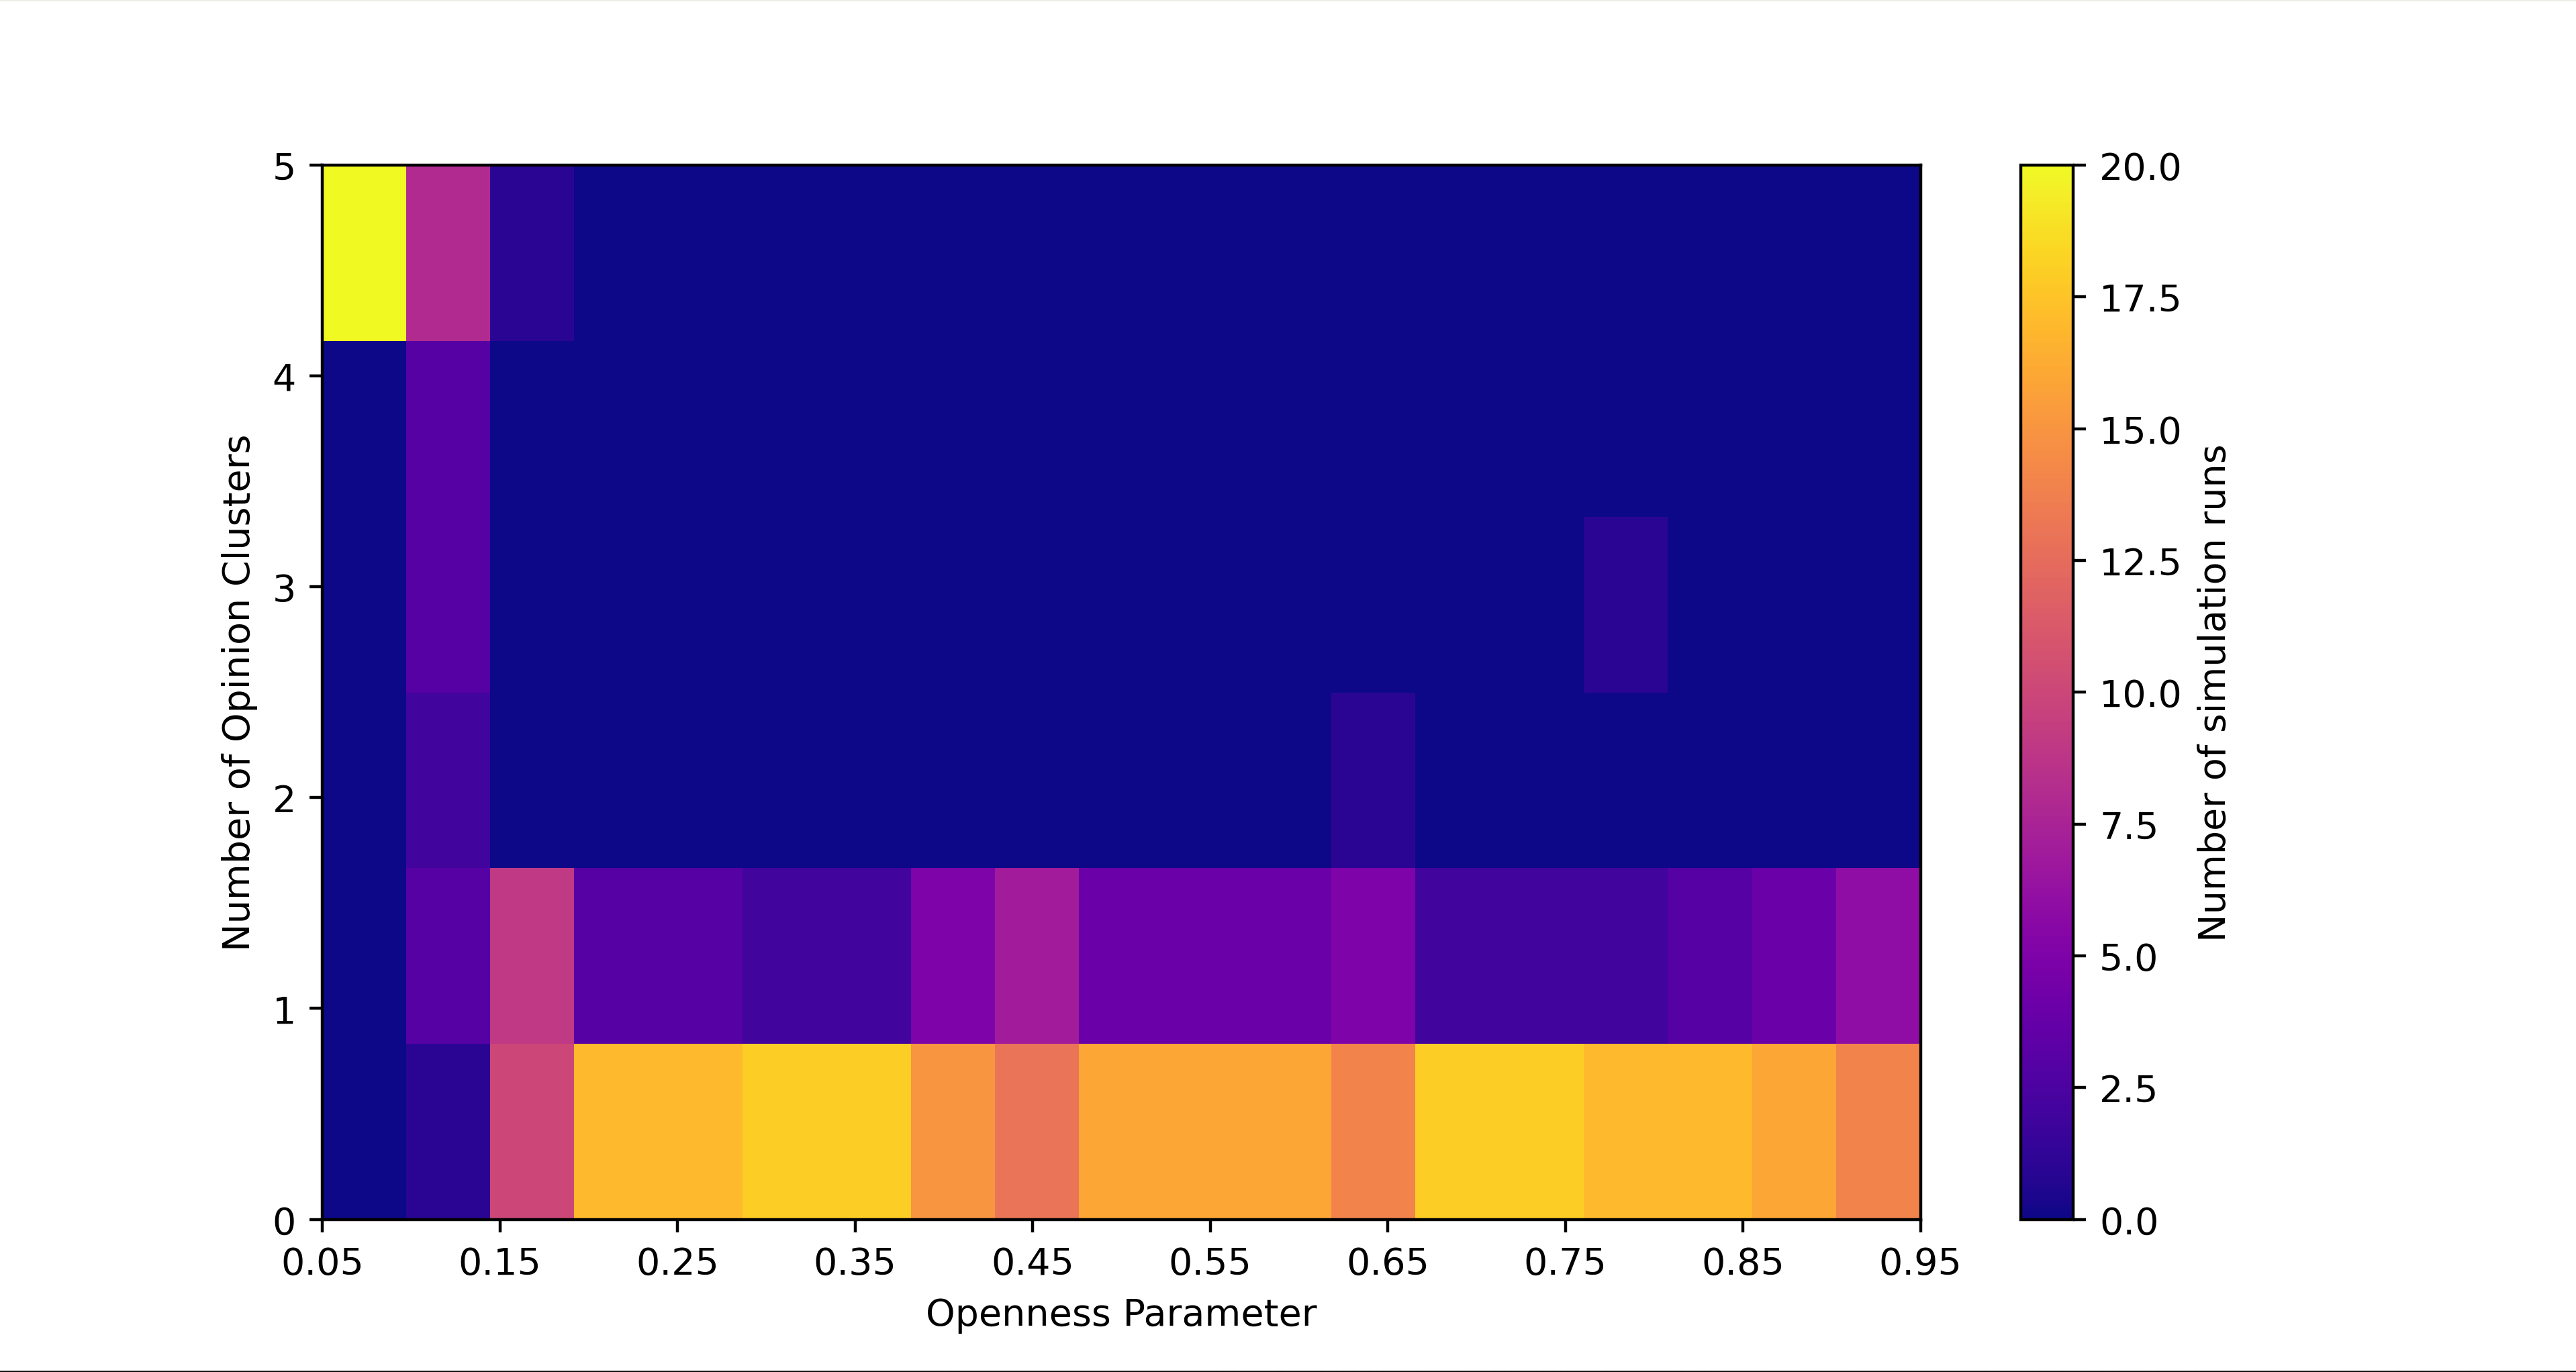
\includegraphics[width=1.0\columnwidth]{./Graphs/Cluster_openBig.png}
\caption{Number of Opinion Clusters and the Openness Parameter (0.05 - 0.95)}
\label{H2b_plot_big}
\end{figure}

We noticed that there was little to no difference between an openness parameter
of 0.5 and 0.7. However, we observed that the openness parameter had more
impact on the number of opinion clusters when the parameter was closer to 0.10.
To further explore this result, we ran another parameter sweep with 50 agents,
5 issues, an edge probability of 0.50, and a suite size of 20. This time, we
varied the openness parameter from 0.05 to 0.40. Our results are depicted in
Figure~\ref{H2b_plot_small}.

\begin{figure}
\centering
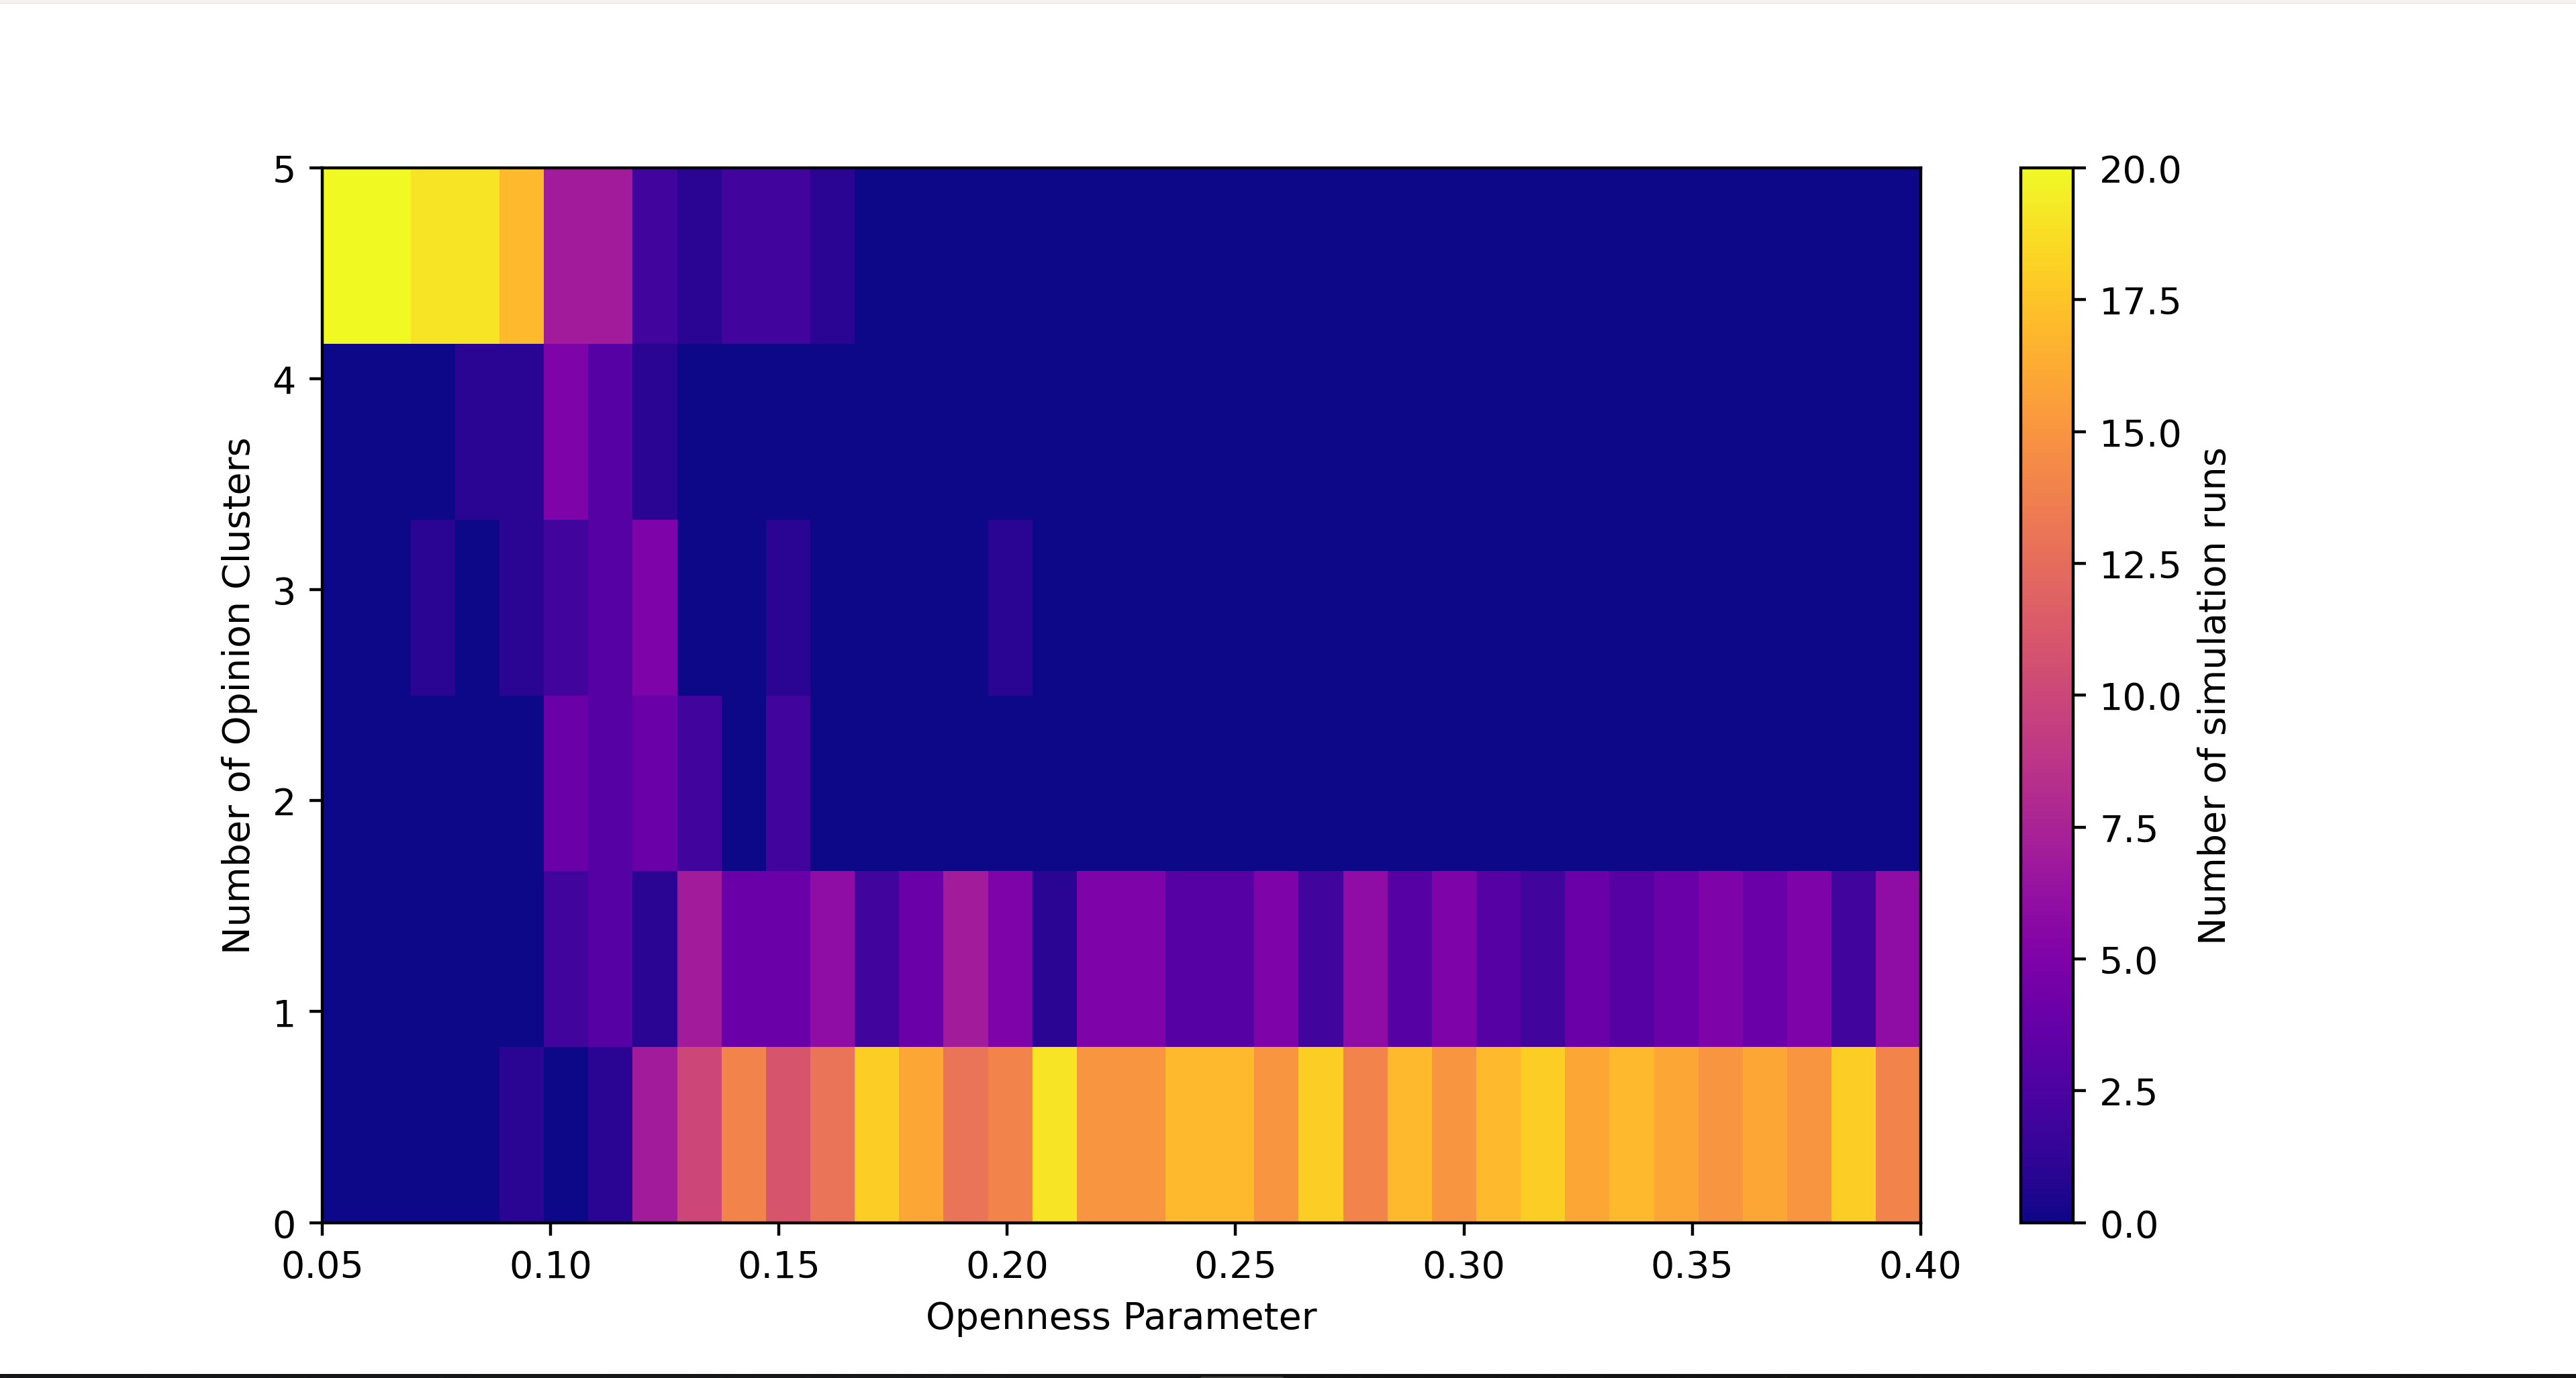
\includegraphics[width=1.0\columnwidth]{./Graphs/Cluster_opensmall.png}
\caption{Number of Opinion Clusters and Openness (0.05 - 0.40)}
\label{H2b_plot_small}
\end{figure}

This graph indicates that there is a tipping point for the openness parameter.
When the openness for agents in the model is very low, the agents did not agree
on many issues. However, as Figure~\ref{H2b_plot_small} indicates, when we
increase the openness parameter slightly, the number of opinion clusters across
the model quickly drops. As a result, we can infer that low levels of openness
in a society may induce more polarized societies. When agents in the model are
less open to distant opinions, there are more opinion clusters for any given
issue. However, the tipping point leads us to believe that slightly higher
levels of openness are sufficient to reach uniformity on a given issue for all
agents in the model. To conclude, when using the cross-issue influence
mechanism, marginally higher levels of openness led to to less polarization in
the model.

